%!TEX root=rapport.tex
\section{Implémentation}

\subsection{Idée générale}

	L'idée générale de l'alignement de séquences est de permettre, à partir d'un ensemble de séquences, de créer à l'aide de chevauchements approximatifs un \emph{contig}. Pour ce faire, notre démarche se découpe en plusieurs parties:

	\begin{description}
		\item[Récupération et stockage des données] Afin de pouvoir former le contig souhaité, il est nécessaire de récupérer les séquences et de les stocker de manière efficace. Cette étape est expliquée dans la section~\ref{subsection:recStock}.

		\item[1.Alignement semi-global] Ensuite, pour chaque paire de séquences,
			nous effectuons un \emph{alignement semi-global} en nous inspirant
			de l'algorithme vu en cours. Cette méthode nous donne ainsi
			les chevauchements approximatifs des deux séquences, ce qui permet de
			prendre en compte le fait qu'il ait pu y avoir des erreurs lors du
			séquençage. Si la paire est notée $(s, t)$, cette étape nous permet également de connaitre la plus
			grande chaine qui est suffixe de $s$ et préfixe de $t$ (à erreurs de séquençage près). Cette étape
			est expliquée dans la section~\ref{subsection:semiGlobal}.

		\item[2.Algorithme greedy] Une fois les alignements approximatifs
			calculés, il est encore nécessaire de trouver dans quel ordre
			ceux-ci doivent être assemblés afin de former le meilleur contig.
			Pour ce faire, nous utilisons un \emph{algorithme glouton} qui, à
			partir d'un graphe permet de trouver un chemin hamiltonien afin de
			reconstituer le contig. Cette étape est expliquée dans la
			section~\ref{subsection:greedy}.

		\item[3.Alignement]
			L'algorithme glouton nous donnant, dans l'ordre, les séquences à
			aligner, il est nécessaire de reconstruire cet alignement en
			ajoutant des gaps pour que chaque séquence ait la même longueur et
			qu'on puisse calculer le consensus. Cette étape est expliquée dans
			la section ~\ref{subsection:alignment}.

		\item[4.Consensus]
			Après que l'alignement a été réalisé, il nous faut calculer le
			consensus en fonction de ce dernier. Cette étape est expliquée dans
			la section ~\ref{subsection:consensus}.
	\end{description}

\subsection{Récupération et stockage des données}
\label{subsection:recStock}

Des sous-séquences brutes d'ADN sont stockées dans des fichiers au format FASTA, il nous est donc nécessaire de les récupérer. Cette étape est effectuée au travers des classes \verb|FastaReader| et \verb|Sequence|. En effet, la classe \verb|FastaReader| génère une liste de séquences à partir des séquences stockées dans le fichier FASTA. De plus, la classe \verb|FastaWriter| est utilisée afin de récupérer le résultat du procédé visant à trouver le meilleur contig.
\\

La classe \verb|Segment| permet de stocker sous forme d'un tableau d'octets un fragment d'ADN. Nous prenons la convention suivante quant à la représentation des nucléotides et d'un gap:
	\begin{center}
		\begin{tabular}{|l|c|}
			\hline
			Nucléotide/Gap & Représentation \\
			\hline
			\hline
			C & 0 \\
			\hline
			G & 1\\
			\hline
			T &  2 \\
			\hline
			A &  3 \\
			\hline
			Gap & 4 \\
			\hline

		\end{tabular}
	\end{center}

	Le fait de stocker les nucléotides sous forme de Bytes permet de réduire l'espace mémoire nécessaire pour retenir en mémoire une séquence d'ADN. En effet, si nous avions stocké naïvement les séquences sous forme d'un String chaque caractère de la chaîne prendrait 4 octets contre 1 octet les caractères à l'aide d'un byte.

\subsection{Alignement semi-global}
\label{subsection:semiGlobal}

Une des premières étapes de notre démarche est d'effectuer un alignement semi-global
de deux séquences. Le calcul d'une matrice de similarités entre les deux séquences à aligner doit être effectué. A partir de certaines valeurs associées à un gap ( ex: \begin{tabular}{c} A \\ - \end{tabular} ou \begin{tabular}{c} - \\ A \end{tabular} ), à un match (\begin{tabular}{c} A \\ A \end{tabular}) et à un missmatch (\begin{tabular}{c} A \\ C \end{tabular}) celle-ci permet de calculer les différents scores des alignements possibles entre les deux séquences. Dans le cadre d'un alignement semi-global, le score d'alignement correspond à la somme des scores 
Dans le cadre de ce projet, nous utilisons les valeurs suivantes:

\begin{center}
	\begin{tabular}{|l|c|}
		\hline
		 & Valeur \\
		\hline
		\hline
		match & 1 \\
		\hline
	 	missmatch & -1\\
		\hline
		gap &  -2 \\
		\hline
	\end{tabular}
\end{center}





 L'alignement semi-global est implémenté dans la classe \verb|Sequence| via la fonction \emph{semiGlobalAlignement} qui utilise la fonction \emph{computeSimMat} et \emph{backTrack}. Cette méthode prend deux séquences $f$ et $g$, les coûts de match, missmatch et gap et calcule l'alignement dont le score d'alignement est le plus élevé et  tel que $f$ précède $g$ - nous appelons cet alignement un alignement de type ($f,g$) - et celui tel que $g$ précède $f$ - nous appelons cet alignement un alignement de type ($g,f$)- et renvoie le résultat sous la forme d'une liste de \verb|SequenceAlignement|. Ce comportement est un différent de celui du cours, car dans ce dernier on se contentait de garder le meilleur des deux alignements du point de vue du score d'alignement. Ici nous sommes intéressés à la fois  au meilleur alignement suffixe-prefixe de $f$ avec $g$ mais également le cas inverse ($g$ avec $f$). Ces deux situations sont illustrés à la figure~\ref{fig:alignementType}.
On remarque que lorsque l'on calcule la matrice de similarité, si le fragment $f$ est placé sur l'axe vertical et si le fragment $g$ est placé sur l'axe horizontal, on trouve le score d'alignement de type $(f,g)$ en prenant le maximum sur la dernière ligne de la matrice. En effet, cela signifie que l'on a parcouru tous les éléments de la séquence $f$ avant de finir le parcours des éléments de la séquence $g$. De la même manière on trouve les alignements de type $(g,f)$ en prenant le maximum de la dernière colonne de la matrice.\\

\begin{figure}
	\begin{minipage}[r]{.46\linewidth}
		\begin{center}
		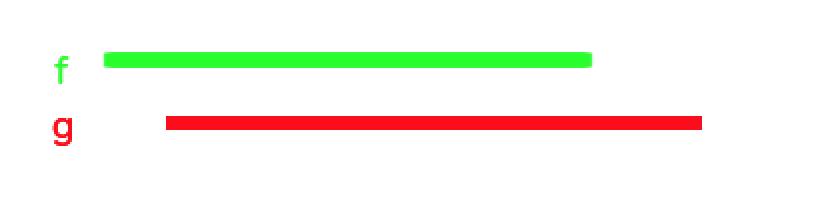
\includegraphics[scale= 0.50]{(f,g).png}
		Alignement de type (f,g)
	\end{center}
	   \end{minipage} \hfill
	   \begin{minipage}[c]{.46\linewidth}
		\begin{center}
			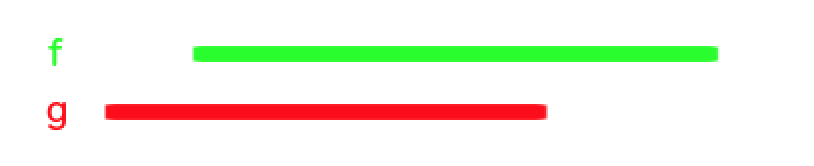
\includegraphics[scale= 0.50]{(g,f).png}
			Alignement de type (g,f)
		\end{center}
			  \end{minipage}
		\caption{Résultats de l'alignement de f et de g}
		\label{fig:alignementType}
\end{figure}


Un objet de la classe \verb|SequenceAlignement| est défini de la manière
suivante: le fragment $f$ aligné (stocké dans l'argument \emph{s1}) avec le segment $g$ (stocké dans l'argument \emph{s2}) en supposant que le
segment $f$ est le segment le plus à \og gauche \fg.

De plus,  dans la classe \verb|Sequence| nous retrouvons la méthode \emph{arcGenerator} qui à partir de deux fragments $f$ et $g$ calcule les alignements suivants:\\
\begin{itemize}
	\item[$\bullet$] Les alignements $(f,g)$ et $(g,f)$;
	\item[$\bullet$] Les alignements $(\overline{f},g)$ et $(g, \overline{f})$;
	\item[$\bullet$] Les alignements $(f, \overline{g})$ et $(\overline{g},f)$;
	\item[$\bullet$] Les alignements  $(\overline{f}, \overline{g})$ et $(\overline{g}, \overline{f})$.
\end{itemize}
Où $\overline{f}$ est le fragment complémentaire inversé de $f$.\\
Au vu des explications ci-dessus, il est important de remarquer que pour trouver les 8 alignements il n'est nécessaire de calculer uniquement 4 matrices de similarités (une pour chaque paire de l'énumération ci-dessus).\\

A partir de ces alignements, nous représentons les relations entre toutes les paires d'alignement sous la forme d'arcs. Un arc possède les attributs suivants:\\

\begin{itemize}
	\item[$\bullet$] Les fragments $f$ et $g$ initiaux qui sont utilisés lors de l'alignement. Ceux-ci sont stockés dans les attributs \emph{start} et \emph{end} qui représentent respectivement l'origine et de l'extrémité de l'arc.
	\item[$\bullet$] Des booléens relatifs à $f$ et $g$ - respectivement \emph{startComp} et \emph{endComp} qui permettent de savoir si on considère le complémentaire inversé lors de l'alignement.
	\item[$\bullet$] Le score correspondant à l'alignement.
	\item[$\bullet$] Un booléen \emph{inside} qui permet de déterminer si, lors de l'alignement, un des deux fragments est inclus à l'autre.
	
\end{itemize}

Nous pouvons remarquer que nous ne stockons pas, l'alignement résultant de l'alignement semi-global. En effet, comme à la fin du procédé le nombre d'alignements réels qui nous intéressent sont au nombre de $n-1$ (si $n$ est le nombre de fragments), il n'est pas nécessaire de stocker en mémoire tous les alignements possibles. Dans le but de gagner en mémoire, nous préférons dès lors recalculer l'alignement correspondant aux arcs choisis par l'algorithme greedy. Ceci est réalisé par le biais de la méthode \emph{getAlignement} de la classe \verb|Arc|.

Ces arcs nous permettent d'effectuer l'algorithme greedy pour trouver un chemin hamiltonien parcourant tous les fragments considérés.


\subsection{Algorithme greedy}
\label{subsection:greedy}

Avant de nous intéresser à l'algorithme greedy en tant que tel, nous allons expliquer une structure de données \emph{Union-Find} que nous utilisons pour l'implémentation de cet algorithme.

\subsubsection{Union-Find}

Une structure de donnée \og Union-Find \fg~est une structure permettant de représenter une relation d'équivalence . On peut effectuer trois opérations sur cette structure:
\begin{itemize}
\item[$\bullet$] L'opération \textsc{Find} permet de déterminer dans quelle classe d'équivalence se situe un élément.
\item[$\bullet$] L'opération \textsc{Union} permet de faire l'union entre deux classes d'équivalence.
\item[$\bullet$] L'opération \textsc{MakeSet} construit une classe d'équivalence qui ne contient qu'un seul élément
\end{itemize}

Dans l'implémentation que nous avons utilisée, chaque classe d'équivalence est représentée par un arbre pour lequel chaque noeud possède une référence vers son père. Dans un tel choix d'implémentation, la racine de chaque classe correspond au représentant de la classe d'équivalence.

L'idée est que l'opération \textsc{Find} permet de retourner à la racine de l'arbre et donc de déterminer quel est le représentant de la classe d'équivalence. Pour l'opération \textsc{Union}, on rattache la racine d'une des deux classes à celle de l'autre classe. Toutefois, une telle démarche pourrait amener à des arbres fortement déséquilibrés . Afin d'éviter cela, une heuristique sur la hauteur de l'arbre est utilisée. On retient le \emph{rang} de l'arbre et à chaque fois que l'on veut faire l'union de deux arbres on considère leur rang. On attache l'arbre de rang inférieur à la racine de l'arbre de rang supérieur. Les arbres qui ne contiennent qu'un seul élément sont de rang 0 et dès que l'on effectue l'union de deux arbres de même rang, le résultat de cette union a un rang d'une unité plus grand.

La complexité en temps pour les opérations sur cette structure de donnée ont une complexité amortie en $\mathcal{O}(\alpha (n))$ où $\alpha(n)$ est l'inverse de la fonction $n = f(x) = A(x,x)$ où $A$ est la fonction de Ackermann. Cette fonction est une fonction qui croit très vite. En pratique, $\alpha(n)$ vaut moins de 5 pour toute valeur de $n$. Dès lors la complexité amortie des opérations sur Union-Find est en temps constant.

Nous avons basé notre implémentation et nos explications sur la page : \url{https://fr.wikipedia.org/wiki/Union-Find}
\subsubsection{Recherche du chemin hamiltonien}

Afin de trouver la meilleure séquence finale, nous devons trouver un chemin hamiltonien de poids maximal dans le graphe composé des arcs dont la construction est décrite dans la section~\ref{subsection:semiGlobal}. Le déroulement général de l'algorithme greedy est le suivant: à chaque étape d'exécution de l'algorithme, l'algorithme sélectionne et retire l'arc de poids le plus élevés d'un ensemble d'arcs. Plusieurs critères doivent alors être vérifiés pour savoir si l'arc doit être retenu. Si l'arc est l'arc $(f,g)$ où $f$ est l'origine de l'arc et $g$ son extrémité, il faut vérifier qu'on ne soit pas déjà rentré dans le \og noeud \fg~$g$ ni qu'on ne soit déjà sorti du \og noeud \fg~$f$, de plus, il faut s'assurer que $f$ et $g$ ne fasse pas déjà partie de la même classe d'équivalence. Vu que dans notre cas, nous travaillons également avec les complémentaires inversés, il faut s'assurer que lorsqu'un fragment $f$ est choisi pour la formation du chemin hamiltonien, il ne sera plus possible d'utiliser son complémentaire inversé $\overline{f}$.

La mise en oeuvre de l'algorithme greedy se trouve dans la classe \verb|Greedy|. Nous détaillons ci-dessous le rôle des différentes méthodes qui s'y trouvent.

\begin{description}
	\item[\textsc{generateAllPairs}] Cette méthode permet à partir d'une liste d'objets \verb|Sequence| de générer toutes les paires de séquences qui devront être considérées.
	\item[\textsc{isAcceptable}] Pour un arc donné, cette méthode permet de déterminer si cet arc suit les conditions d'acceptabilité expliquées ci-dessus. 
	\item[\textsc{filterArcs}] C'est au sein de cette méthode que l'algorithme greedy comme décrit dans le cours est effectué. A partir d'une liste d'arcs, on calcule les sequences ayant générés ces arcs afin de pouvoir générer la structure d'\verb|Union-find|. Deux ensembles \emph{entered} et \emph{exited} permettent de tenir à jour les \og noeuds \fg~dans lesquels on est rentré ou sorti. Une autre structure \emph{comp} permet de savoir déterminer si on a déjà utilisé un fragment et si oui, s'il est utilisé sous sa forme complémentée inversée ou pas. L'algorithme choisit à chaque fois l'arc de poids le plus élevé et teste s'il est acceptable. Si oui, on ajoute cet arc pour la construction du chemin hamiltonien et on met à jour toutes les structures décrites précédemment et on choisit un nouvel arc. Si non, on choisit directement un nouvel arc.
	\item[\textsc{hamiltonianPath}] A partir de l'ensemble des arcs acceptés par la méthode \emph{filterArcs} reconstruit le chemin hamiltonien sous forme d'une liste d'arcs.
	\item[\textsc{greedy}] Cette méthode rassemble toutes les méthodes précédentes. On commence par générer toutes les paires de séquences possibles. A partir de cela, nous construisons les arcs. C'est à cet endroit que le travail est le plus couteux (car il demande de calculer les matrices de similarité). C'est pourquoi nous parallélisons cette étape. Nous avons ensuite la possibilité de retenir certains arcs selon certains critères. Nous avons tenté de rejeter les arcs qui correspondaient un alignement de type \og inside \fg. Les tests effectués après cette modification semblant donner des résultats moins bons, cette alternative n'a pas été retenue. Nous n'avons dès lors, à ce jour, pas encore trouvé de moyen efficace de traiter les alignements de type \og inside \fg. Nous construisons ensuite le chemin hamiltonien d'arcs. Toutefois, les alignements n'étant pas stocké dans les arcs, nous devons recalculer les alignements entre les deux séquences. Cela se fait via le biais de la fonction \emph{getAlignement} de la classe \verb|Arc|. 
	Ensuite, on renvoie le chemin hamiltonien de \verb|SequenceAlignment| qui est ainsi prêt à être utilisé pour retrouver la séquence finale.	
\end{description}

%!TEX root=rapport.tex

\subsection{Alignement}
\label{subsection:alignment}

Les deux dernières étapes que sont l'alignement et le consensus sont
implémentées dans la classe \verb|ConsensusAbstract| à travers les méthodes
\verb|computeAlignment| qui calcule l'alignement des séquences et le sauvegarde
dans l'attribut \verb|alignment| ainsi qu'à travers la méthode \verb|build|
qui calcule le consensus.

Pour calculer l'alignement, nous utilisons les segments alignés dans l'ordre
donné par l'algorithme greedy décrit à l'étape \ref{subsection:greedy}.
L'algorithme greedy nous ressort une liste de paires de séquences $P_{i}$ tel
que le deuxième segment de la paire $P_{i}$ provient du même segment initial que
le premier de la paire $P_{i + 1}$, la différence se situant dans les gaps
ajoutés lors de l'alignement semi-global entre les nucléotides pour offrir le
meilleur score pour chaque paire.

Pour pouvoir construire le contig final, il nous faut réaligner convenablement
chaque paire de segments et pour cela, nous allons propager les gaps qui ont été
ajoutés lors des calculs de l'alignement semi-global. Nous effectuons cette
propagation en deux temps:

\begin{enumerate}
	\item vers le bas, c'est-à-dire, pour une paire $P_{i}$, on regarde si entre
		deux nucléotides de la deuxième composante de $P_{i}$, le
		nombre de gaps est plus grand qu'entre les deux mêmes nucléotides de la première
		séquence de la paire suivante $P_{i + 1}$ et si c'est le cas, on propage la
		différence entre ces nombres vers les séquences du dessous.
	\item vers le haut par le même procédé que pour la propagation vers le bas
		sauf que nous propageons les gaps qui sont plus présents dans la
		première composante de la paire $P_{i + 1}$ que dans la deuxième
		composante de paire $P_{i}$ et qu'on propage alors la différence de gaps
		vers les séquences du dessus.
\end{enumerate}

Grace à ce procédé, nous sommes sûrs que les séquences résultantes des
alignements semi-globaux sont bien les mêmes et que l'ordre renvoyé par le greedy
est toujours le même (car l'ordre des scores reste le même).

\subsubsection{Représentation d'une séquence pour l'alignement}
\label{subsubsection:repr_sequence_alignment}

Au vu de cette méthode de propagation de gaps, le procédé d'alignement n'est
donc qu'un ajout de gaps entre nucléotides: il est alors intéressant de
représenter les séquences alignées comme des séquences sans gaps où, après
chaque nucléotide de la séquence, nous retenons, dans un tableau d'entier, le
nombre de gaps suivant celui-ci.\footnote{Une même représentation peut être
	utilisée pour représenter pour les nucléotides successifs identiques: nous
	compressons ainsi la séquence. Nous n'avons souhaité compresser que les gaps
	car nous n'allons travailler qu'avec ceux-ci, et cela aurait complexifié
l'implémentation des méthodes.}

Par exemple, la séquence \verb|A--T-G-C| sera représentée par une séquence
\verb|ATGC| et par un tableau nommé \verb|nb_gaps| de taille 4
contenant les entiers {2, 1, 1, 0} car il y a deux gaps après le premier
nucléotide, un gap après le second, un après le troisième, et 0 à la fin. Les
complexités en temps et en mémoire sont ainsi diminuées car la plupart des
algorithmes travaillent avec la séquence initiale.
Au niveau de la mémoire, une séquence alignée se voit ainsi 'compressée' en la
séquence initiale et les gaps ne sont qu'une information supplémentaire ajoutée
à la séquence initiale.

L'ajout de gaps sera alors très simple et très rapide en complexité. En effet,
si nous souhaitons ajouter un gap à la position 2 (supposons qu'on commence à
calculer en 0) à la séquence \verb|A--T-G-C| pour obtenir \verb|A---T-G-C|, il
nous suffira d'augmenter de 1 le nombre de gaps après le nucléotide A: nous
obtiendrons alors le tableau {3, 1, 1, 0}. Cet ajout de gap peut se faire en
$O(n)$ où $n$ est la taille de la séquence \textit{initiale}. De plus,
l'insertion de gaps ne demande pas plus d'espace mémoire: qu'importe si nous
devons insérer $2$ gaps ou $10000$ gaps car nous ne faisons qu'augmenter la case
correspondante du tableau \verb|nb_gaps|. \footnote{Avec la représentation sous
	forme de byte (1 octet en Java), cette nouvelle abstraction est intéressante
si nous devons ajouter plus de 7 gaps entre chaque nucléotide (un entier prenant
8 octets), ce qui peut arriver si nous travaillons sur de grandes séquences.} La
plupart des méthodes ont alors une complexité relative à la taille de la
séquence \textit{initiale}, et non la séquence alignée et vu que l'insertion de
gaps ne modifie jamais la taille de la séquence initiale, nous
gardons toujours une complexité relative à la taille de la séquence initiale, ce
qui est avantageux dans le cas d'insertions de très grands nombres de gaps.

Un autre point positif est qu'il est très facile de connaitre la position où nous
devons insérer des gaps s'il nous est demandé de rajouter $n$ gaps entre deux
nucléotides: il suffit de connaitre la position du nucléotide dans la chaine
initiale après lequel nous devons ajouter les $n$ gaps.

Nous gardons également un attribut contenant l'offset de la séquence dans le
chemin hamiltonien, c'est-à-dire le décalage vers la droite du début de la
séquence. Cela nous amène à parler de position relative et de position absolue.
La position relative d'un élément dans une séquence est la position de l'élément
sans l'offset tandis que la position absolue est la position en prenant compte
de l'offset.

\begin{exemple}
	Soit la séquence \verb|A--T-G-C| et considérons un offset de 4, c'est-à-dire
	que 'réellement', la séquence est \verb|----A--T-G-C|.

	En commençant de calculer à 0, le nucléotide à la position relative 3 est
	\verb|T| tandis que ce même nucléotide est la position absolue $4 + 3 = 7$,
	l'élément à la position absolue 3 étant le dernier gap avant le \verb|A|.
\end{exemple}

Cette distinction est à faire car lorsque nous devons propager des gaps, nous
devons considérer cet offset, c'est-à-dire travailler avec la position absolue.

Par la suite, nous travaillerons toujours avec la position \textit{absolue}.

Cette abstraction des séquences est implémentée dans la classe
\verb|SequenceAbstract|.\footnote{Cela justifie le nom de la classe
	\verb|ConsensusAbstract| qui travaille avec des objets de la classe
\verb|SequenceAbstract|, et non \verb|Squence|.}

Divers constructeurs sont implémentés (pour permettre diverses compatibilités
avec les autres parties et si nous souhaitons améliorer le projet) mais un seul
est utilisé dans \verb|ConsensusAbstract|: celui qui demande un objet de la
classe \verb|Sequence| représentant une séquence alignée.  L'algorithme, en
$O(n)$ où $n$ est la taille de la séquence alignée, reconstruit la séquence
initiale et le tableau de gaps, l'offset étant mis à la position du premier
nucléotide.

Les autres méthodes utilisées sont:
\begin{description}
	\item[\textsc{getSize}]: Récupère la taille de la séquence. La taille est
		contenue dans un attribut \verb|size| qui est mis à jour à chaque fois
		qu'on ajoute des éléments et cette mise à jour se fait en O(1). Cette
		implémentation permet de garder une complexité en O(1) et de diminuer la
		complexité de \verb|addEndGaps| dans \verb|ConsensusAbstract| par
		exemple.
	\item[\textsc{complement}]: Construit, en $O(m)$ avec $m$ la taille de la
		séquence \textit{initiale}, le complémentaire inversé de la séquence.
		Cette méthode est donc plus rapide que la méthode \verb|complement| de
		\verb|Sequence| qui nécessite de parcourir toute la séquence
		\textit{alignée}.
	\item[\textsc{addGapsAndReturnIndice}]: insère $n$ gaps à
			une position (absolue) donnée et retourne l'indice (dans la séquence
			initiale) du nucléotide après lequel les gaps ont été insérés, le
			tout en $O(m)$ où $m$ est la taille de la séquence initiale. Le
			retour de la fonction est utile pour la propagation entre deux
			séquences provenant d'une même séquence initiale quand on doit
			connaître entre quels nucléotides nous avons inséré les gaps.
	\item[\textsc{addGapsAfterIndiceAndReturnPosition}]: insère $n$ gaps après
		le nucléotide se trouvant à l'indice donné dans la séquence initiale.
		Cette méthode est utilisée quand nous devons propager des gaps entre
		deux séquences ne provenant pas de la même séquence initiale et que nous
		devons connaitre alors la position où les gaps ont été insérés. La
		complexité est également en $O(m)$ où $m$ est la taille de la séquence
		initiale.
\end{description}

\subsubsection{Propagation des gaps}

Comme expliqué précédemment, la propagation des gaps se fait en deux temps: vers
le bas puis vers le haut.

Les méthodes s'occupant de la propagation se trouvent dans la classe
\verb|ConsensusAbstract|.

Avant tout, en se rappelant que le chemin hamiltonien qui nous est renvoyé ne
tient pas compte de l'offset, il faut le calculer. La méthode
\verb|computeOffset| s'occupe, en $O(k)$ où $k$ est la longueur du chemin
hamiltonien, de mettre à jour les offsets des séquences du chemin en alignant
les séquences provenant de la même séquence initiale, c'est-à-dire, pour deux
paires $P_{i}$ et $P_{i + 1}$, la deuxième séquence de $P_{i}$ va être alignée
(ie le premier nucléotide va être placé au même décalage) avec la première
séquence de $P_{i + 1}$.

Viennent les propagations des gaps.
Les méthodes s'en chargeant sont
\verb|propageGapsDownFrom| et \verb|propageGapsUpFrom|. Les algorithmes étant
sensiblement les mêmes pour le bas et le haut, nous décrivons uniquement la
propagation vers le bas.

Dans \verb|computeAlignment|, nous parcourons chaque paire $P_{i}$ du chemin
hamiltonien et faisons appel à \verb|propageGapsDownFrom| en envoyant comme
paramètre l'indice $i$. Comme expliqué précédemment, il faut regarder la
séquence $t_{i}$ se trouvant en seconde position dans la paire $P_{i}$ et celle en
première position de la paire $P_{i + 1}$, notée $s_{i + 1}$, et parcourir chaque nucléotide en
propageant vers le bas la différence de gaps (nous rappelons que $t_{i}$ et
$s_{i + 1}$ proviennent de la même séquence initiale et ont donc les mêmes
nucléotides, la différence se situant dans le nombre de gaps entre
chaque) si $t_{i}$ comporte plus de gaps que $s_{i + 1}$.

S'il y a plus de gaps dans $t_{i}$ que dans $s_{i + 1}$ entre les
nucléotides $n_{j}$ et $n_{j + 1}$, ce que nous pouvons savoir en $O(1)$ grace à
la nouvelle abstraction des séquences car il suffit de comparer le tableau des
gaps à la position $j$, nous propageons la différence vers le bas.
Cette propagation se fait à travers la méthode
\verb|propageGapsDownFromPosition| (resp. \verb|propageGapsUpFromPosition|) qui
prend deux paramètres: l'indice et le nombre de gaps à propager.

Cette dernière méthode parcourt, à partir de la paire $P_{i} = (s_{i}, t_{i})$,
toutes les paires $P_{j} = (s_{j}, t_{j})$, $i < j \leq n$ et ajoute les $n$
gaps nécessaires dans les segments $s_{j}$ et $t_{j}$. Supposons que nous devons
propager $n$ gaps venant d'entre les nucléotides $n_{k}$ et $n_{k + 1}$ de
$t_{i}$, c'est-à-dire que nous devons insérer dans $s_{i + 1}$ après l'indice
$k$.

L'insertion se fait de manière récursive sur $j$:
\begin{itemize}
	\item[$\bullet$] Pour $j = i + 1$, c'est-à-dire la paire juste après $P_{i}$, nous
		devons insérer les gaps entre les deux nucléotides $n_{k}$ et $n_{k +
		1}$ de $s_{i + 1}$. Cette insertion se fait grâce à la méthode
		\verb|addGapsAfterIndiceAndReturnPosition| sur $s_{i + 1}$ (en $O(m)$,
		$m$ étant la taille de la séquence initiale d'où provient $t_{i}$) et on
		récupère en plus la position absolue d'insertion (ce qui provoque le $m$
		dans la complexité de la méthode car nous devons calculer à la volée la
		position absolue). Cette position absolue va permettre de savoir où il
		faut propager les gaps dans la séquence $t_{i + 1}$. Grace à cette
		position, on utilise la méthode \verb|addGapsAndReturnIndice| sur $t_{i
		+ 1}$ pour insérer les gaps où il faut, et nous récupérons en même temps
		l'indice du nucléotide de $t_{i + 1}$ après lequel les gaps ont été
		ajoutés. Cette dernière méthode est également en $O(m)$, toujours pour
		la même raison que précédemment.
	\item[$\bullet$] Pour $j > i + 1$, nous répétons l'opération du cas de base mais cette
		fois-ci, nous utilisons l'indice que la méthode
		\verb|addGapsAndReturnIndice| nous a renvoyé à l'étape $j - 1$.
\end{itemize}

Pour un appel à \verb|propageGapsUpFromPosition|, nous obtenons donc une
complexité en $O( (k - i) M_{i})$ où $M_{i}$ est la taille de la plus grande
séquence du chemin, $k$ le nombre initial de séquence et $i$ la position de
début de l'insertion.

Cela entraine donc une complexité en $O( (k - i) M_{i}^{2})$ pour
\verb|propageGapsDownFrom| car nous faisons appel, pour chaque nucléotide de
$t_{i}$ (dans le pire des cas), à la méthode \-\verb|propageGapsUpFromPosition|.
Par conséquence, comme \verb|propageGapsDown| parcourt toutes les paires en
faisant appel à \verb|propageGapsDown|, nous obtenons une complexité finale de
$O(k^{2} M_{i}^{2})$.

Pour simplifier le calcul du consensus à la dernière étape, nous mettons à jour
les gaps finaux des séquences pour que toutes les séquences aient la même
longueur. Ce calcul est fait par \verb|addEndGaps| et se déroule en $O(k)$ où
$k$ est le nombre initial de séquences. Cette méthode se charge de calculer la
taille de la plus longue séquence (en $O(k)$ car \verb|getSize| est en $O(1)$)
et elle ajoute le nombre de gaps dans le tableau \verb|nb_gaps| pour chaque
séquence. Ce nombre de gaps à ajouter à la séquence courante est égale à la
taille maximale moins la taille de la séquence courante.

Pour l'ensemble de la méthode \verb|computeAlignment|, on obtient donc une
complexité de

\begin{equation}
	\overbrace{O(k)}^{\text{ mise à jour offset}} + \overbrace{2 O(k^{2}
	M_{i}^{2})}^{\text{propagation haut et bas}} + \overbrace{O(k)}^{\text{ajout
	des gaps finaux}} = O(k^{2} M_{i}^{2})
\end{equation}

%TODO: exemple de propagation. En trouver un avec 3 séquences initiales pour
%montrer que la propagation ne se fait pas en colonne.
%\begin{center}
	%- - AT - - G - - C - -
%\end{center}

\subsection{Consensus}
\label{subsection:consensus}

Grace à l'alignement précédemment réalisé, nos paires $P_{i}$ et $P_{i + 1}$ ont
maintenant la même séquence respectivement en deuxième composante et en première
composante et toutes les séquences sont maintenant bien alignées. Pour
construire le contig final, nous allons parcourir chaque colonne de l'alignement
et prendre le nucléotide qui apparait le plus souvent. En cas d'égalité, nous
prenons par ordre alphabétique.

Pour parcourir les objets de la classe \verb|SequenceAbstract|, nous avons
implémenté un itérateur sur ceux-ci qui permet d'avoir un algorithme clair et
dont la complexité est en $O(k M_{i})$ où $k$ est le nombre initial de
séquences et $M_{i}$ la taille de la plus longue séquence.

\begin{comment}

\subsection{Deuxième approche}

Dans cette section nous expliquons l'approche du calcul de la séquence finale exposé par Aline.
L'idée est un peu différente, car au contraire de l'approche précédente, nous ne propageons pas physiquement les gaps mais travaillons sur les paires d'alignements en les parcourant de gauche à droite chacune à leur tour. Chaque paire d'alignement n'étant pas de la même longueur ni parfaitement alignés les uns en dessous des autres, il faut savoir se rappeler à quelle position de la séquence finale nous nous trouvons réellement lors du traitement. C'est ici que l'idée d'\emph{offset} intervient. Cette méthode nécessite un nouvel objet \verb|Counter| qui est un compteurr  permettant de retenir pour chaque colonne le nombre de $A$, de $C$, de $T$ et de $G$ qui ont été comptabilisés en une certaine position (pour un certain compteur) de la séquence finale. Une fois tous les compteurs récupérés pour toutes les positions de la séquence finale il suffit de récupérer le nucléotide ayant comptabilisé le maximum d'occurrences pour cette colonne.

Un premier test de l'implémentation de cette idée a été effectué sans tenir compte du fait que des gaps pouvaient apparaitre au sein même d'un alignement. Par exemple si on a l'alignement de $(f,g)$ puis celui de $(g,h)$, il se peut que les gaps internes au niveau de $g$ dans le premier alignement ne soient pas les mêmes que les gaps internes de $g$ au niveau du second alignement.
Nous avons pour cela besoin d'un dictionnaire qui a un entier (une position possible dans la séquence finale) associe un compteur et de la notion d'offset.

Pour mieux comprendre la notion d'offset, illustrons-la sur la situation de la figure~\ref{offset}. Lors du parcours de première paire d'alignement, l'offset est à 0 car $f$ est à gauche de $g$. On parcourt alors toutes les positions des deux alignements en créants de nouveaux compteurs car il n'en existe pas encore pour les positions couvertent par $f$ et $g$.
Lorsqu'on va traiter l'alignement $(g,f)$ l'offset devient négatif car le nucléotide le plus à gauche à traiter est avant le nucléotide que l'on avait considérer comme étant en position 0 (le premier nucléotide de la séquence $f$). On parcourt alors cet alignement de la gauche vers la droite sachant que pour certaine position (celles déjà couvertent par l'alignement $(f,g)$) des compteurs existent déjà et qu'il nous suffit donc de les mettre à jour.
\begin{figure}
		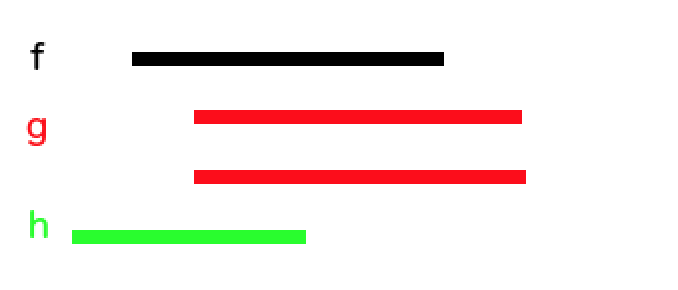
\includegraphics[scale= 0.50]{offset.png}
		\caption{Deux paires d'alignement $(f,g)$ et $(g,f)$}
		\label{fig:offset}
\end{figure}

Une telle approche, plutôt naïve, fournit déjà des résultats plutôt satisfaisants.
\end{comment}

